\documentclass[journal]{IEEEtran}

\usepackage{amsmath,amsfonts}
\usepackage{graphicx}
\usepackage{booktabs}
\usepackage{array}
\usepackage{multirow}
\usepackage{cite}
\usepackage{url}
\usepackage{hyperref}

\newcommand{\hlif}{HyperLIF}
\newcommand{\adhlif}{Adaptive HyperLIF}
\newcommand{\lif}{LIF}
\newcommand{\plif}{PLIF}
\newcommand{\alif}{ALIF}
\newcommand{\apex}{APEX}

\begin{document}

\title{HyperLIF Learning: A Controlled Cross-Framework Study of a Continuous-Reset Spiking Neuron}

\author{Anonymous Author(s)%
\thanks{Manuscript submitted for review. Author names and affiliations withheld for blind review.}}

\markboth{Submitted to IEEE Journal, 2026}{Anonymous \MakeLowercase{\textit{et al.}}: HyperLIF Learning}

\maketitle

\begin{abstract}
Leaky integrate-and-fire neurons remain attractive for efficient temporal computation, but thresholding and hard reset make them hybrid non-smooth systems. We study \hlif, a continuous-reset spiking neuron in which a fast gate controls reset conductance. The continuous state path removes the reset jump; the threshold-event observable remains non-differentiable and still requires a surrogate or event-time derivative when it participates in the loss. The goal is mechanistic isolation rather than benchmark optimization. Across event datasets, readouts, and feedforward, convolutional, recurrent, and learnable-delay architectures, \hlif{} improves most strongly on temporal speech and motion tasks while its advantage shrinks on the near-static N-MNIST control. Gate-only readouts show that the \hlif{} gate is a decodable task state for which \lif{} has no homologous variable. Contemporary \plif{} and \alif{} baselines show a nuanced picture: \alif{} is a serious competitor on SHD-wide shortlists, while \hlif{} remains competitive and often stronger in recurrent cells. Finally, a byte-identical Julia/\apex{} validation reproduces a small tuned \hlif{} advantage over matched dense \lif{} on SHD after gate-feedback calibration. Historical architecture runs also expose a threshold-occupancy-versus-accuracy dial, but their HyperLIF observable counts above-threshold samples rather than upward crossings; physical spike-count and energy claims are therefore deferred pending a semantics-matched rerun. These results support \hlif{} as a mechanistically interpretable temporal-learning and state-readout mechanism, with clearly bounded limitations in deep residual spiking stacks.
\end{abstract}

\begin{IEEEkeywords}
Spiking neural networks, leaky integrate-and-fire neurons, surrogate gradients, neuromorphic learning, temporal learning, event-based vision, SHD, N-MNIST.
\end{IEEEkeywords}

\section{Introduction}
\IEEEPARstart{S}{piking} neural networks (SNNs) promise temporal, sparse, and hardware-aligned computation, but the standard leaky integrate-and-fire (\lif) neuron is a hybrid non-smooth system: threshold emission is discontinuous in state and the reset overwrites the membrane. These two operations are distinct. Removing the reset jump does not make the binary event map differentiable; event-dependent training still needs a surrogate derivative or explicit event-time sensitivity \cite{Neftci2019Surrogate,Zenke2018SuperSpike}.

\hlif{} replaces the hard reset with a continuous, gate-controlled reset conductance. A fast gate tracks threshold proximity and smoothly modulates the reset, turning a state jump into a differentiable internal trajectory. This paper asks a deliberately narrow question: when architecture, optimizer, data split, and readout family are controlled, does the neuron itself improve temporal learning, expose useful state, and reproduce across implementations?

The contribution is a controlled mechanistic study rather than a benchmark competition. We make six claims. First, \hlif{} gains are temporal-specific: large on speech and motion streams, small on N-MNIST. Second, the gate is a decodable state that \lif{} lacks. Third, adaptive reset conductance creates an operating dial between sampled threshold occupancy and accuracy; a physical event-efficiency claim requires a crossing-matched rerun. Fourth, the effect transfers to convolutional, recurrent, and learnable-delay cells but is bounded by a deep residual failure case. Fifth, \plif{} \cite{Fang2021PLIF} and \alif{}/LSNN \cite{Bellec2018LSNN} baselines sharpen the claim: \hlif{} does not universally dominate adaptive neurons, but it remains a strong temporal and state-rich mechanism. Sixth, a Julia/\apex{} reproduction on byte-identical SHD caches confirms a calibrated cross-framework \hlif{} advantage over matched dense \lif{}.

\section{Related Work}
SNN learning has been advanced by surrogate-gradient BPTT \cite{Neftci2019Surrogate,Zenke2018SuperSpike}, local learning rules such as e-prop \cite{Bellec2020Eprop}, and adaptive neuron families such as LSNN/\alif{} \cite{Bellec2018LSNN} and \plif{} \cite{Fang2021PLIF}. These methods largely retain a hard reset while adapting thresholds, time constants, or learning rules. \hlif{} instead changes the reset mechanism itself, turning the spike-associated reset into a continuous conductance process.

Event datasets such as N-MNIST \cite{Orchard2015NMNIST} and SHD \cite{Cramer2022SHD} provide complementary stress tests. N-MNIST has a stereotyped saccade structure and often saturates under simple models, while SHD and speech command data require stronger temporal integration. This distinction is central to our experimental design: the paper treats N-MNIST as a near-static control rather than as the only benchmark target.

\section{Neuron Model}
The \hlif{} state consists of a membrane voltage $v$ and gate $r$. In continuous form, the implemented dynamics are
\begin{align}
\tau_v \dot v &= -(v - v_{\mathrm{rest}}) + I - G(r, I)(v - v_{\mathrm{reset}}),\\
\tau_r \dot r &= \sigma\left(\alpha(v-\theta_{\mathrm{eff}})\right) - r,\\
\theta_{\mathrm{eff}} &= \theta - \gamma r.
\end{align}
For plain \hlif{}, $G(r,I)=g_{\mathrm{reset}}r^2$. For \adhlif{}, the reset conductance is input-modulated,
\begin{equation}
G(r,I) = \left(G_{\mathrm{base}} + \beta |I|\right)r^2.
\end{equation}
The gate therefore acts as both a continuous reset variable and a candidate readout state. The parameter $\gamma$ controls gate feedback on threshold, $\beta$ controls drive-dependent reset conductance, and $\tau_r$ controls gate memory.

In the PyTorch/snnTorch arm, the neuron is implemented as a two-state module with readouts over spikes, membrane, gate, and conductance features. In the Julia/\apex{} arm, the same concept is implemented by a microstep GPU kernel with a `use\_nsa' switch that selects the continuous \hlif{} update rather than the \lif{} control. The final \apex{} validation uses the same SHD HDF5 cache as the PyTorch runs.

\section{Experimental Design}
\subsection{Controlled Isolation}
The central isolation principle is fixed architecture and varied neuron/readout. The base model is a shallow temporal SNN with a 256-unit spiking layer and a linear classifier. The architecture-transfer sweep repeats the neuron/readout comparison in convolutional, recurrent, and learnable-delay models.

\begin{table}[t]
\centering
\caption{Dataset and factor scope. N-MNIST is treated as a near-static control; speech and gesture streams form the temporal stress tests.}
\label{tab:datasets}
\begin{tabular}{llll}
\toprule
Dataset & Modality & Classes & Role \\
\midrule
SHD & speech spikes & 20 & high temporal \\
SSC & speech spikes & 35 & high temporal \\
DVS-32 & event gesture & 11 & motion temporal \\
DVS-48 & event gesture & 11 & motion temporal \\
N-MNIST & event vision & 10 & near-static control \\
\bottomrule
\end{tabular}
\end{table}

\subsection{Baselines and Metrics}
The core comparison uses \lif{}, \hlif{}, and \adhlif{}. The reviewer-facing baseline extension adds \plif{} and \alif{}/LSNN cells. Metrics are test accuracy, macro-F1 where available, the historically logged threshold-output total per sample, stability, and cross-framework reproducibility. For \hlif{}/\adhlif{} in the architecture harness this total is sampled occupancy $\sum_k\mathbf{1}[v_k\geq\theta_e]$, not the upward-crossing count $\sum_k\mathbf{1}[v_{k-1}<\theta_e\leq v_k]$ used by the standalone/Nengo reference. Consequently it is retained as a diagnostic but not interpreted as physical spike count or energy. A run is counted only if it completes without NaN instability.

\section{Results}
\subsection{Temporal-Specific Learning Gain}
Figure~\ref{fig:temporal-gain} and Table~\ref{tab:ff-temporal} summarize the feedforward controlled sweep. \hlif{} improves over \lif{} on every temporal dataset, with the largest gains on speech and gesture streams. On N-MNIST, the gain shrinks to approximately one point, which supports the interpretation that \hlif{} is not a generic accuracy booster but a temporal-learning mechanism.

\begin{figure}[t]
\centering
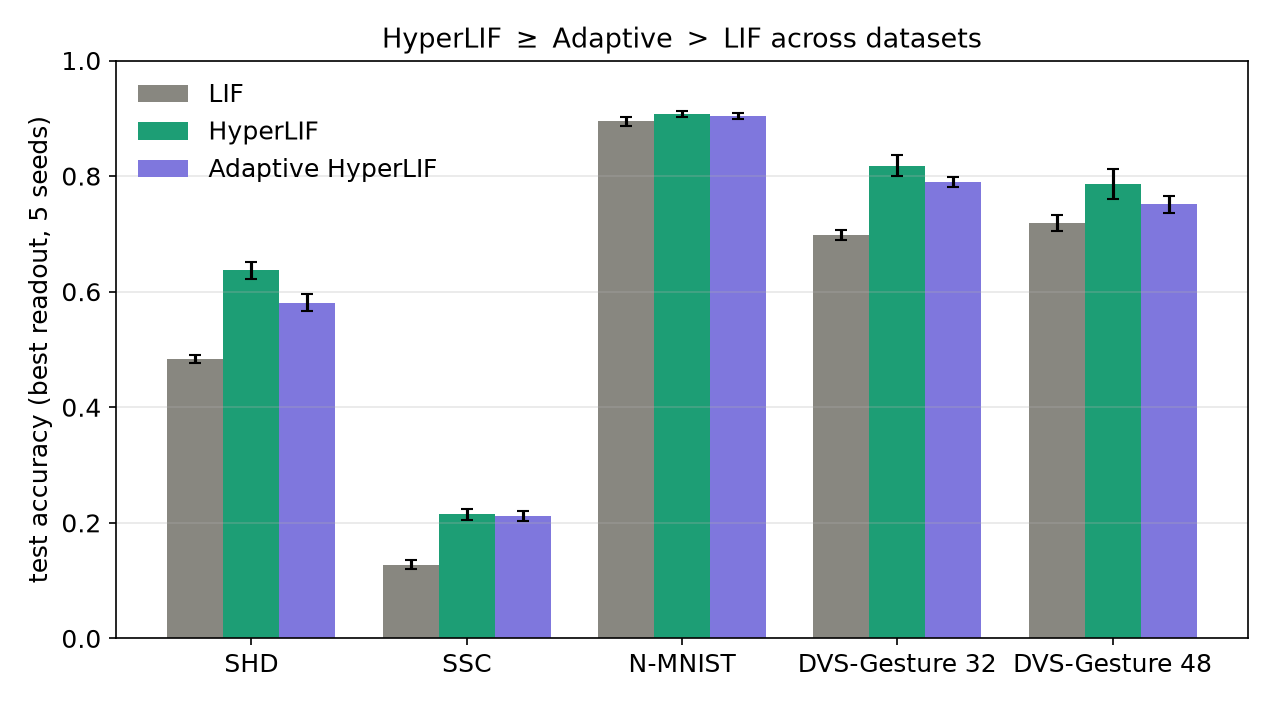
\includegraphics[width=\linewidth]{figures/fig1_best_per_neuron.png}
\caption{Best readout per neuron in the feedforward controlled sweep. Gains are largest on temporal speech and motion data and smallest on N-MNIST.}
\label{fig:temporal-gain}
\end{figure}

\begin{table}[t]
\centering
\caption{Feedforward controlled result, best readout per neuron. Values are mean test accuracy $\pm$ sample standard deviation over five seeds; all selected rows had zero failures and zero NaN batches.}
\label{tab:ff-temporal}
\footnotesize
\begin{tabular}{lccc}
\toprule
Dataset & \lif{} & \hlif{} & \adhlif{} \\
\midrule
SHD & $0.484{\pm}0.008$ & $\textbf{0.637}{\pm}0.016$ & $0.581{\pm}0.016$ \\
SSC & $0.128{\pm}0.008$ & $\textbf{0.215}{\pm}0.010$ & $0.212{\pm}0.010$ \\
DVS-32 & $0.698{\pm}0.010$ & $\textbf{0.818}{\pm}0.020$ & $0.790{\pm}0.010$ \\
DVS-48 & $0.719{\pm}0.016$ & $\textbf{0.786}{\pm}0.030$ & $0.751{\pm}0.016$ \\
N-MNIST & $0.895{\pm}0.009$ & $\textbf{0.908}{\pm}0.007$ & $0.904{\pm}0.006$ \\
\bottomrule
\end{tabular}
\end{table}

\subsection{Gate State as a Decodable Signal}
Figure~\ref{fig:gate-state} and Table~\ref{tab:gate-readout} show the mechanism result. A gate-only readout is structurally blind for \lif{}, because \lif{} exposes no comparable continuous gate state. The same readout remains strongly predictive for \hlif{}. This is a useful falsification test: if the gate were only a numerical artifact, gate-only \hlif{} should also collapse.

\begin{figure}[t]
\centering
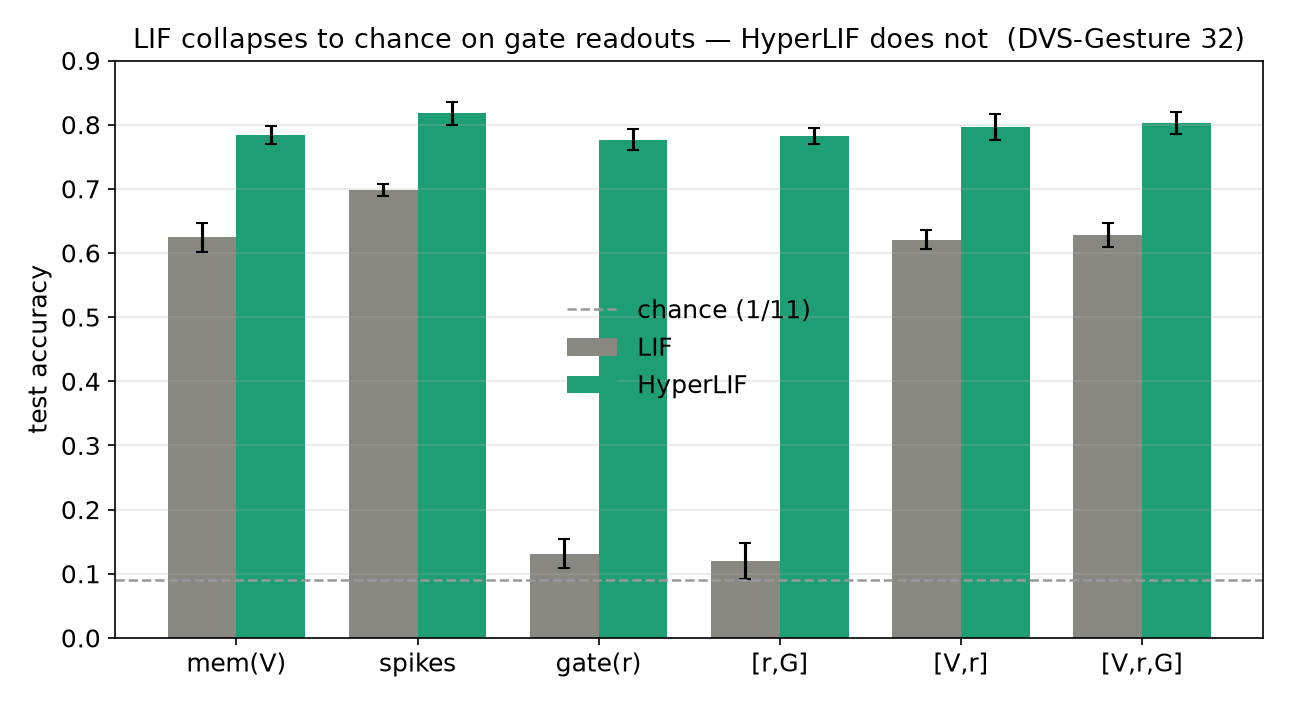
\includegraphics[width=\linewidth]{figures/fig2_structural_blindness.png}
\caption{Gate-readout structural blindness. Gate-only and gate-conductance readouts collapse for \lif{} but remain informative for \hlif{}.}
\label{fig:gate-state}
\end{figure}

\begin{table}[t]
\centering
\caption{DVS-32 readout comparison on identical wiring. Chance is $1/11=0.091$.}
\label{tab:gate-readout}
\begin{tabular}{lcc}
\toprule
Readout & \lif{} & \hlif{} \\
\midrule
spike count & 0.698 & \textbf{0.818} \\
membrane & 0.624 & 0.784 \\
hybrid $[\bar v,\bar r]$ & 0.621 & 0.796 \\
hybrid $[\bar v,\bar r,\bar G]$ & 0.628 & 0.803 \\
gate $\bar r$ & $0.131 \pm 0.023$ & $\textbf{0.776} \pm 0.017$ \\
gate-conductance & $0.120 \pm 0.028$ & $\textbf{0.782} \pm 0.013$ \\
\bottomrule
\end{tabular}
\end{table}

\subsection{Efficiency Dial}
The adaptive conductance term lets the model move along a threshold-occupancy-versus-accuracy curve. Figure~\ref{fig:efficiency-shallow} shows the shallow setting; Fig.~\ref{fig:efficiency-arch} shows large reductions in logged occupancy in selected convolutional settings. This is an operating-point diagnostic, not yet an event-driven energy result, because the compared neuron families do not share crossing semantics.

\begin{figure}[t]
\centering
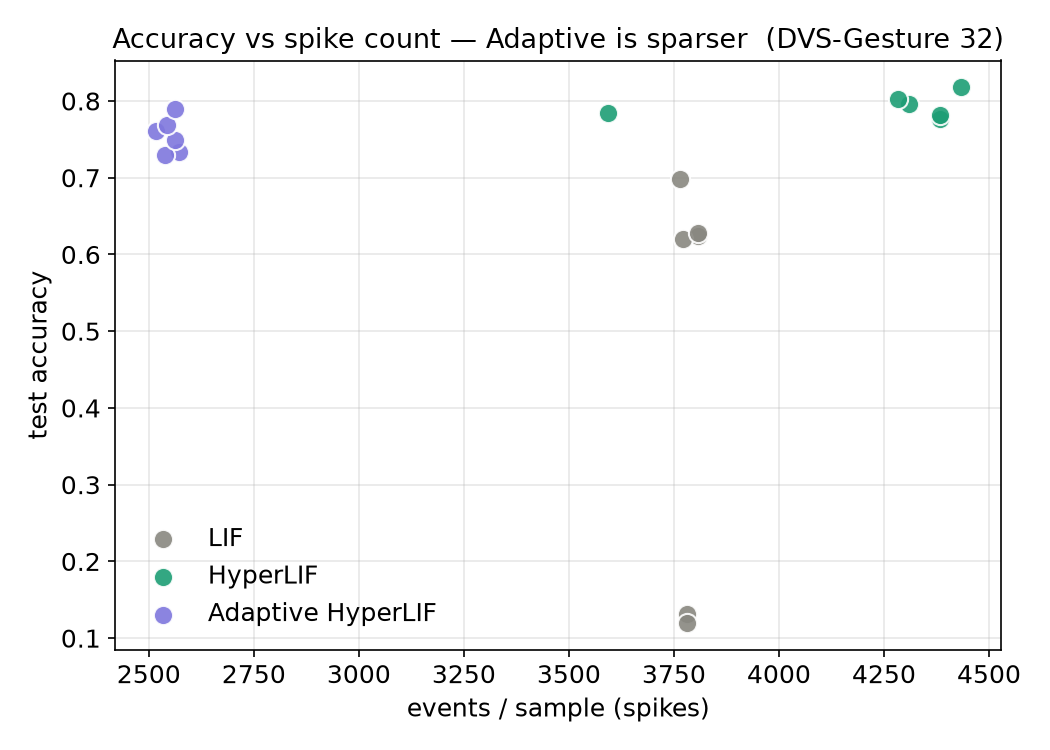
\includegraphics[width=\linewidth]{figures/fig3_efficiency_pareto.png}
\caption{Shallow threshold-occupancy-versus-accuracy diagnostic. The logged HyperLIF quantity counts above-threshold samples, so it is not yet a semantics-matched spike Pareto.}
\label{fig:efficiency-shallow}
\end{figure}

\subsection{Architecture Transfer and Boundary}
Table~\ref{tab:arch-transfer} and Fig.~\ref{fig:architecture-gap} show that the \hlif{} advantage transfers across convolutional, recurrent, and learnable-delay cells. The strongest gaps occur where temporal structure is most important. The claim is bounded: in the current deep residual spiking configuration, \hlif{} does not train reliably and appears limited by deep gradient propagation rather than by simple firing density.

\begin{figure*}[t]
\centering
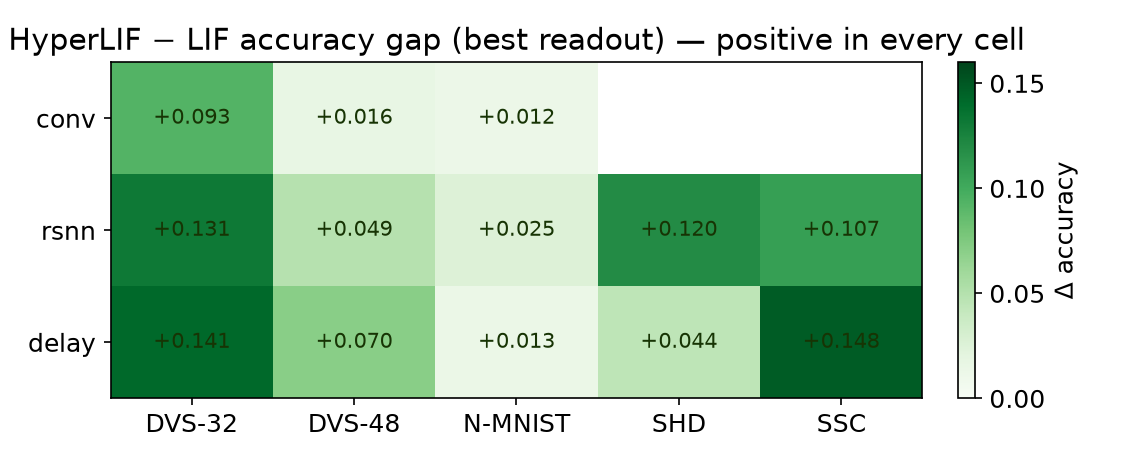
\includegraphics[width=0.82\textwidth]{figures/fig4_arch_transfer_gap.png}
\caption{Architecture-transfer gap. \hlif{} improves over \lif{} across the tested convolutional, recurrent, and delay cells, with the largest gains in temporal datasets.}
\label{fig:architecture-gap}
\end{figure*}

\begin{table*}[t]
\centering
\caption{Architecture-transfer result, best readout per neuron. Values are mean test accuracy $\pm$ sample standard deviation over five seeds; all selected rows had zero failures and zero NaN batches.}
\label{tab:arch-transfer}
\footnotesize
\begin{tabular}{llcccc}
\toprule
Architecture & Dataset & \lif{} & \hlif{} & Gap & \adhlif{} \\
\midrule
conv & DVS-32 & $0.769{\pm}0.010$ & $0.851{\pm}0.016$ & +0.082 & $\textbf{0.854}{\pm}0.027$ \\
conv & DVS-48 & $0.759{\pm}0.021$ & $0.776{\pm}0.017$ & +0.016 & $\textbf{0.785}{\pm}0.011$ \\
conv & N-MNIST & $0.932{\pm}0.005$ & $\textbf{0.939}{\pm}0.008$ & +0.007 & $0.934{\pm}0.011$ \\
rsnn & DVS-32 & $0.689{\pm}0.031$ & $\textbf{0.814}{\pm}0.014$ & +0.125 & $0.812{\pm}0.025$ \\
rsnn & DVS-48 & $0.714{\pm}0.020$ & $\textbf{0.786}{\pm}0.029$ & +0.073 & $0.769{\pm}0.028$ \\
rsnn & N-MNIST & $0.886{\pm}0.014$ & $\textbf{0.912}{\pm}0.006$ & +0.026 & $0.903{\pm}0.007$ \\
rsnn & SHD & $0.536{\pm}0.014$ & $\textbf{0.674}{\pm}0.009$ & +0.138 & $0.588{\pm}0.027$ \\
rsnn & SSC & $0.116{\pm}0.004$ & $\textbf{0.230}{\pm}0.009$ & +0.114 & $0.211{\pm}0.008$ \\
delay & DVS-32 & $0.686{\pm}0.015$ & $\textbf{0.834}{\pm}0.011$ & +0.149 & $0.798{\pm}0.015$ \\
delay & DVS-48 & $0.712{\pm}0.025$ & $0.797{\pm}0.026$ & +0.085 & $\textbf{0.805}{\pm}0.032$ \\
delay & N-MNIST & $0.899{\pm}0.014$ & $\textbf{0.908}{\pm}0.004$ & +0.009 & $0.898{\pm}0.006$ \\
delay & SHD & $0.655{\pm}0.008$ & $\textbf{0.703}{\pm}0.009$ & +0.048 & $0.655{\pm}0.009$ \\
delay & SSC & $0.138{\pm}0.010$ & $\textbf{0.308}{\pm}0.015$ & +0.170 & $0.258{\pm}0.010$ \\
\bottomrule
\end{tabular}
\end{table*}

\begin{figure}[t]
\centering
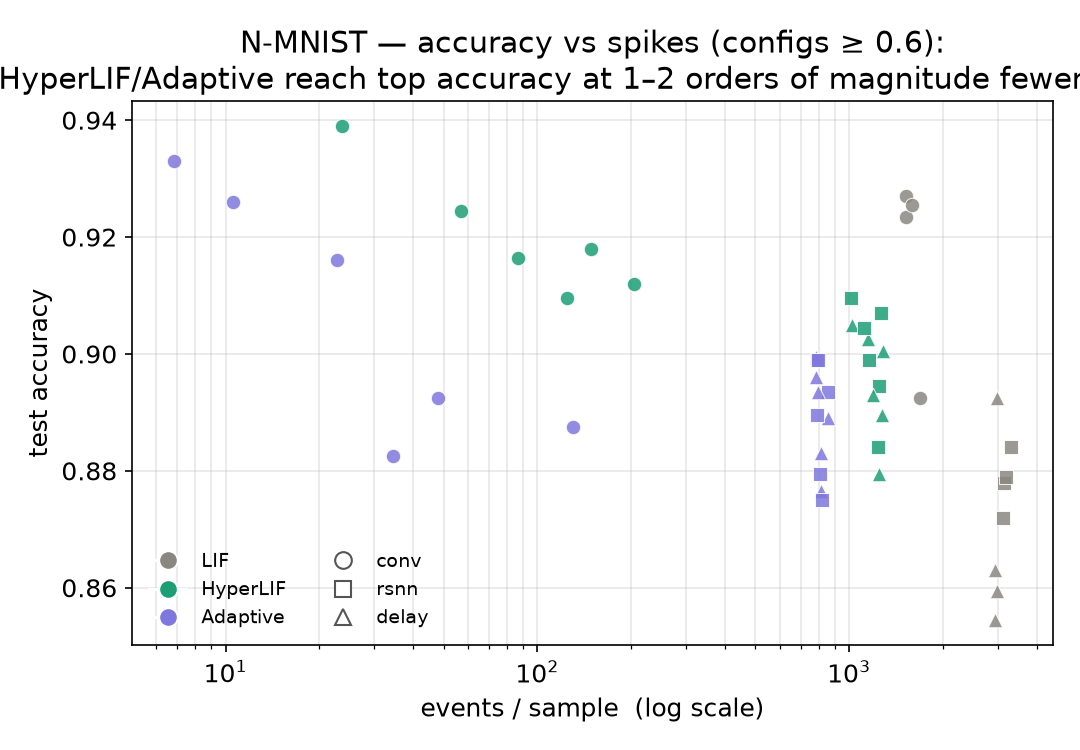
\includegraphics[width=\linewidth]{figures/fig5_efficiency_pareto.png}
\caption{Architecture-scale threshold-output diagnostic. In selected convolutional settings, \hlif{} and \adhlif{} have lower sampled threshold occupancy; physical event and energy conclusions require recomputation with common upward-crossing semantics.}
\label{fig:efficiency-arch}
\end{figure}

\subsection{Reviewer Baselines: PLIF and ALIF}
Table~\ref{tab:baseline-shortlist} addresses the baseline critique directly. \alif{} is not a weak control; it slightly leads the feedforward and delay SHD-wide shortlists. \hlif{} leads the recurrent SHD-wide cell and remains substantially above \lif{}/\plif{}. This supports a nuanced claim: \hlif{} is competitive with adaptive-threshold baselines and exposes a unique decodable gate state, but it does not universally dominate \alif{}.

\begin{table*}[t]
\centering
\caption{Contemporary baseline extension. Accuracy values are mean $\pm$ sample standard deviation over five seeds; all selected rows had zero failures and zero NaN batches. Events/sample are shown to preserve the efficiency interpretation.}
\label{tab:baseline-shortlist}
\footnotesize
\begin{tabular}{llccc}
\toprule
Setting & Model/readout & Accuracy & Events/sample & Status \\
\midrule
N-MNIST tiny FF & \hlif{} hybrid\_vr & $\textbf{0.8975} \pm 0.0070$ & 342.9 & top mean \\
N-MNIST tiny FF & \alif{} hybrid\_vr\_conductance & $0.8967 \pm 0.0192$ & 323.3 & tied competitor \\
N-MNIST tiny FF & \plif{} hybrid\_vr & $0.8750 \pm 0.0106$ & 581.9 & LIF-like \\
N-MNIST tiny FF & \lif{} hybrid\_vr & $0.8742 \pm 0.0123$ & 578.5 & control \\
\midrule
SHD-wide FF & \alif{} hybrid\_vr\_conductance & $\textbf{0.5570} \pm 0.0199$ & 830.2 & top mean \\
SHD-wide FF & \hlif{} hybrid\_vr & $0.5475 \pm 0.0227$ & 1042.2 & close second \\
SHD-wide FF & \lif{} hybrid\_vr & $0.4238 \pm 0.0133$ & 1208.7 & control \\
SHD-wide FF & \plif{} hybrid\_vr & $0.4235 \pm 0.0119$ & 1210.3 & control \\
\midrule
SHD-wide RSNN & \hlif{} hybrid\_vr & $\textbf{0.5695} \pm 0.0172$ & 1035.0 & top mean \\
SHD-wide RSNN & \alif{} hybrid\_vr\_conductance & $0.5473 \pm 0.0179$ & 818.8 & competitor \\
SHD-wide RSNN & \lif{} hybrid\_vr & $0.4640 \pm 0.0091$ & 1186.7 & control \\
SHD-wide RSNN & \plif{} hybrid\_vr & $0.4637 \pm 0.0096$ & 1189.3 & control \\
\midrule
SHD-wide delay & \alif{} hybrid\_vr\_conductance & $\textbf{0.5650} \pm 0.0209$ & 840.6 & top mean \\
SHD-wide delay & \hlif{} hybrid\_vr & $0.5593 \pm 0.0154$ & 1033.2 & close second \\
SHD-wide delay & \lif{} hybrid\_vr & $0.4945 \pm 0.0215$ & 1185.7 & control \\
SHD-wide delay & \plif{} hybrid\_vr & $0.4940 \pm 0.0228$ & 1191.1 & control \\
\bottomrule
\end{tabular}
\end{table*}

\subsection{Cross-Framework Validation in Julia/APEX}
The first \apex{} validation run showed that the SHD cache could train end-to-end, but the default \hlif{}/NSA setting did not exceed \lif{}. We therefore exposed the gate-feedback parameter and ran a compact tuning sweep. Stronger gate feedback, $\gamma=0.80$ with $\beta=0.10$, recovered the expected direction. The final 10-epoch, 5-seed direct comparison is shown in Table~\ref{tab:apex-validation}. This is not the headline benchmark table; it is a calibrated cross-framework reproduction and mechanism check.

\begin{table}[t]
\centering
\caption{Julia/\apex{} validation on byte-identical SHD-wide HDF5 cache. Dense \lif{} and tuned dense \hlif{}/NSA use the same architecture and batches.}
\label{tab:apex-validation}
\begin{tabular}{lcc}
\toprule
Model & Test accuracy & Test loss \\
\midrule
\lif{} control & $0.2411 \pm 0.0778$ & 2.3359 \\
Tuned \hlif{}/NSA & $\textbf{0.2490} \pm 0.0666$ & \textbf{2.2768} \\
\bottomrule
\end{tabular}
\end{table}

We also built an \apex{}-v2 portability layer to separate implementation fidelity from the older native \apex{} architecture choices. \apex{}-v2 directly mirrors the PyTorch dense, recurrent, and temporal-current delay cores, including the $[\bar v,\bar r]$ hybrid readout used in the successful PyTorch architecture table. Table~\ref{tab:apex-v2-traceability} summarizes the validation ladder. These results are used as traceability evidence, not as an additional accuracy benchmark.

\begin{table}[t]
\centering
\caption{\apex{}-v2 PyTorch-to-Julia traceability on SHD-wide. The trunk is fixed for G4--G5; only the readout head is trained.}
\label{tab:apex-v2-traceability}
\footnotesize
\begin{tabular}{@{}>{\raggedright\arraybackslash}p{0.16\linewidth}>{\raggedright\arraybackslash}p{0.38\linewidth}>{\raggedright\arraybackslash}p{0.35\linewidth}@{}}
\toprule
Gate & Scope & Outcome \\
\midrule
G1--G2 & forward traces & 54/54 finite rows \\
G3 & one-batch readout & loss $4.0835 \rightarrow 1.7929$ \\
Shared weights & \hlif{} dense/RSNN/delay & error $\leq 1.05{\times}10^{-5}$ \\
Shared weights & \adhlif{} dense/RSNN/delay & error $\leq 5.09{\times}10^{-4}$ \\
G5 & 3-seed preflight & stable, 0 NaN batches \\
\bottomrule
\end{tabular}
\end{table}

\section{Discussion}
The results support a coherent interpretation: a continuous reset turns the spike-adjacent state into a computational variable. The gate is decodable, the benefit is strongest on temporal tasks, and the adaptive conductance changes both state occupancy and accuracy. The \alif{} comparison is valuable because it prevents a weak-baseline story. \hlif{} should be presented as a different mechanism, not as a universal replacement for adaptive-threshold neurons. Event-efficiency language remains provisional until all cells are evaluated with one crossing definition and on a measured hardware cost model.

The \apex{} result also sharpens the reproducibility claim. Cross-framework agreement is not automatic: the default \apex{} gate-feedback setting underperformed. After calibration, however, tuned \hlif{}/NSA exceeds matched dense \lif{} with lower loss. The paired negative-default and positive-tuned outcomes make the validation more informative than a single successful execution check.

The \apex{}-v2 ladder adds a complementary engineering result: when the PyTorch recurrent and delay recipes are ported directly, their forward values reproduce in Julia under shared weights, and fixed-trunk readout learning remains stable across three seeds. We therefore keep \apex{}-v2 as traceability rather than as the main accuracy evidence.

\section{Limitations}
This paper intentionally uses controlled, often shallow or short-horizon experiments. Absolute accuracies are therefore below highly optimized benchmark systems. The deep residual convres case remains a real limitation: \hlif{} did not train reliably there under the current setup, even with denser event thresholds. Adaptive \hlif{} should be framed primarily as an efficiency operating point until more settings show accuracy gains. Finally, the native \apex{} result is a calibrated dense-cell validation, not a replacement for the PyTorch architecture tables. Native \apex{} recurrent and delay architecture-family preflights run end-to-end, but the older recurrent and fixed-delay paths should remain limitations. \apex{}-v2 closes the forward-portability gap for PyTorch-style recurrent and temporal-current delay cores, but its current training evidence is a bounded fixed-trunk/readout-head preflight rather than a paper-grade multi-epoch accuracy result.

\section{Conclusion}
\hlif{} replaces the \lif{} hard reset with a continuous gate-controlled reset while retaining a non-smooth event readout. Under controlled experiments, that change produces a temporal-specific learning gain, a decodable internal state, and a calibrated cross-framework reproduction. Historical threshold-occupancy totals motivate, but do not yet establish, an event-efficiency claim because they are not semantics-matched to upward-crossing spike counts. The evidence supports a careful conclusion: \hlif{} is a strong temporal and state-readout mechanism, contemporary adaptive baselines remain serious competitors, and the Julia/\apex{} validation is bounded but positive.

\section*{Acknowledgment}
Funding, advisor acknowledgments, compute resources, and repository links will be inserted before submission.

\bibliographystyle{IEEEtran}
\bibliography{refs}

\end{document}
